	\setcounter{num}{10}\setcounter{numz}{0}
	\null\vfill\null	
	\begin{tabularx}{\textwidth}{lllll}		
		& Deutsch 	& Japanisch 	& Kanji &\multirow{13}{*}{\qquad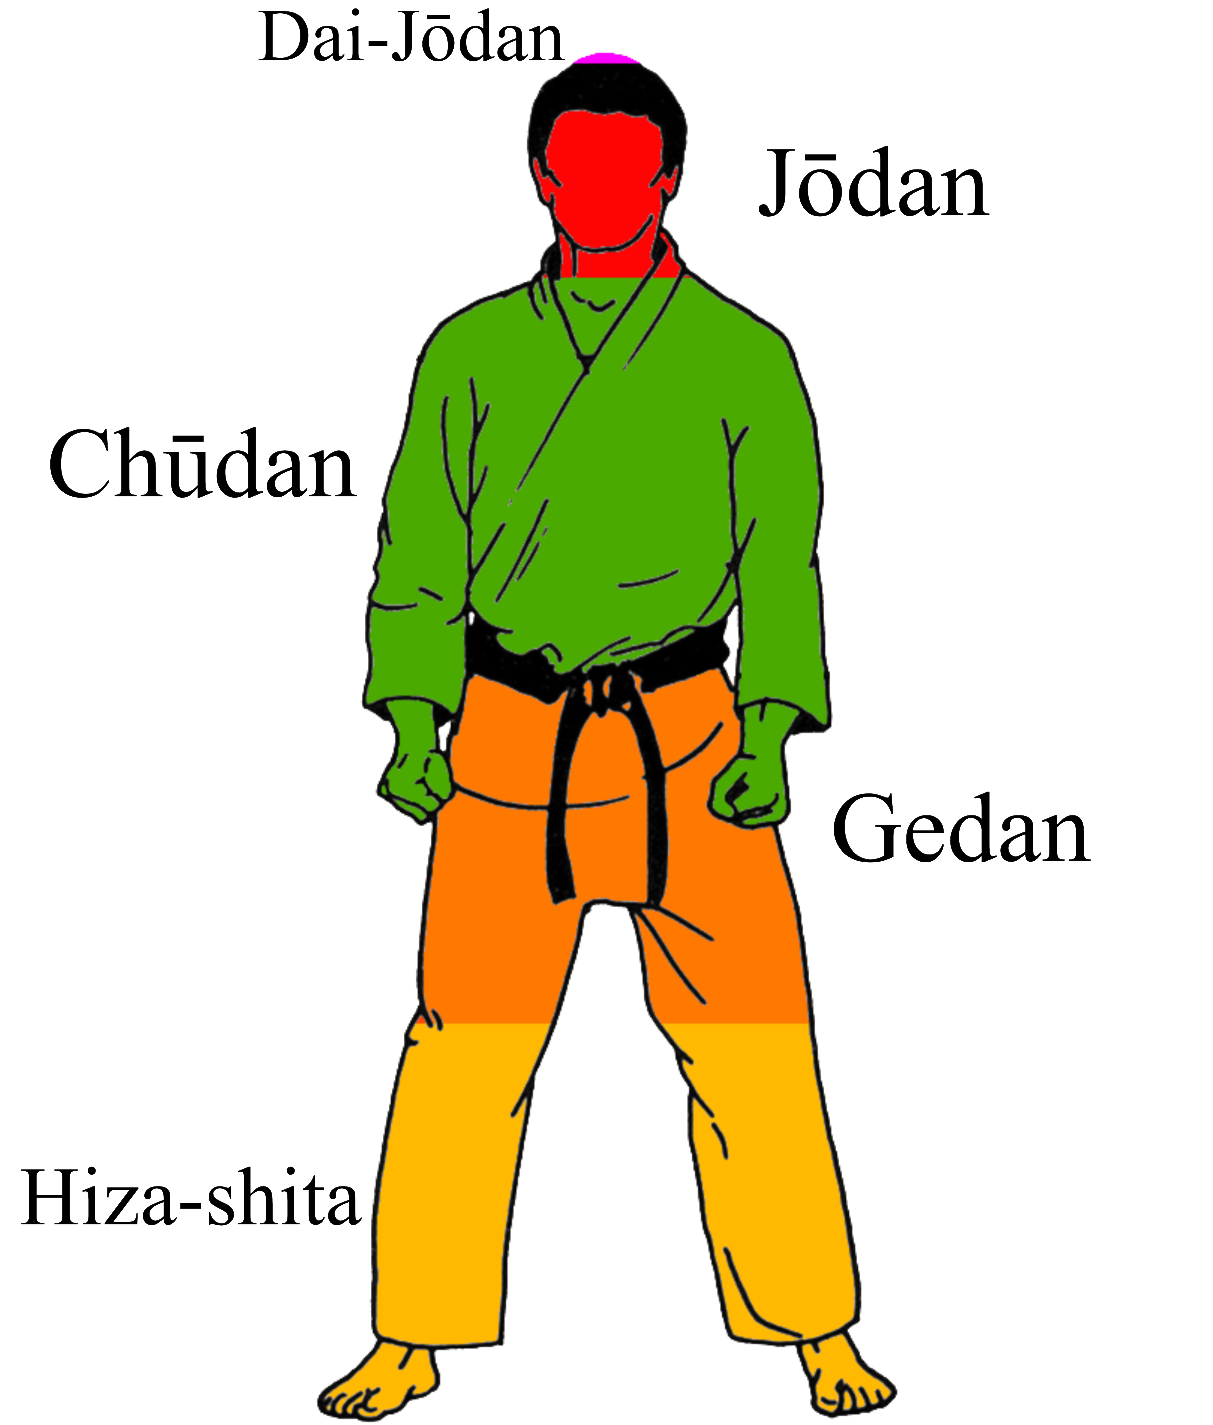
\includegraphics[height=190pt,keepaspectratio]{habersetzer_angriffsstufen_farbig}}\\
		\cmidrule{2-4}
		\ctuz 	& Eins 				& Ichi 					& \begin{CJK*}{UTF8}{ipxm}\color{Navy}一\end{CJK*} 	& \\
		\ctuz 	& Zwei 				& Ni 					& \begin{CJK*}{UTF8}{ipxm}\color{Navy}二\end{CJK*} 	& \\ 
		\ctuz 	& Drei 				& San 					& \begin{CJK*}{UTF8}{ipxm}\color{Navy}三\end{CJK*} 	& \\
		\ctuz 	& Vier 				& Shi 					& \begin{CJK*}{UTF8}{ipxm}\color{Navy}四\end{CJK*} 	& \\
		\ctuz 	& Fünf 				& Go 					& \begin{CJK*}{UTF8}{ipxm}\color{Navy}五\end{CJK*} 	& \\
		\ctuz 	& Sechs 			& Roku 					& \begin{CJK*}{UTF8}{ipxm}\color{Navy}六\end{CJK*} 	& \\
		\ctuz 	& Sieben 			& Shichi 				& \begin{CJK*}{UTF8}{ipxm}\color{Navy}七\end{CJK*} 	& \\
		\ctuz 	& Acht 				& Hachi 				& \begin{CJK*}{UTF8}{ipxm}\color{Navy}八\end{CJK*} 	& \\
		\ctuz 	& Neun 				& Ky\={u} 					& \begin{CJK*}{UTF8}{ipxm}\color{Navy}九\end{CJK*} 	& \\
		\ctuz 	& Zehn 				& J\={u} 					& \begin{CJK*}{UTF8}{ipxm}\color{Navy}十\end{CJK*} 	& \\
		\addlinespace\addlinespace\addlinespace\addlinespace\addlinespace
		& \multicolumn{2}{l}{G\={o}j\={u}-Ry\={u}}	& {\LARGE \begin{CJK*}{UTF8}{ipxm}\color{GKD}剛\,柔\,流\end{CJK*}}        & \\ 	
		& \multicolumn{2}{l}{Karate-D\={o}}			& {\LARGE \begin{CJK*}{UTF8}{ipxm}空\,手\,道\end{CJK*}}        & \\
	\end{tabularx}
	\null\vfill\null